\chapter{Theoretical background}

\section{Mapping}
\label{sec:mapping_operator}
%\sasha
%mapping scheme ($c_{Ii}$ coefficients) \\
%TO DO: picture \\
%translation invariance \\
%definition of the mass \\
%definition of specific and involved atoms \\

The mapping is an operator that establishes a link between the atomistic and coarse-grained representations of the system. An atomistic system is described by specifying the values of the Cartesian coordinates and momenta
\begin{eqnarray}
\bm r^n &=& \{\bm r_1,\dots,\bm r_n\}, \\
\bm p^n &=& \{\bm p_1,\dots,\bm p_n\}.
\end{eqnarray}
of the $n$ atoms in the system.\footnote{In what follows we adopt notations of ref.~\cite{Noid:2008.1}.}
%
On a coarse-grained level, the coordinates and momenta are specified by the positions and momenta of CG sites
\begin{eqnarray}
\bm R^N = \{\bm R_1,\dots,\bm R_N\}, \\
\bm P^N = \{\bm P_1,\dots,\bm P_N\}.
\end{eqnarray}
Note that capitalized symbols are used for the CG sites while lower case letters are used for the atomistic system.

The mapping operator ${\bm c}_I$ is defined by a matrix for each bead $I$ and links the two descriptions
\begin{eqnarray}
 {\bm R}_I &=& \sum_{i=1}^{n}c_{Ii}\bm r_i, \\
 {\bm P}_I &=&
 	M_I \dot{{\bm R}}_I =
	M_I \sum_{i=1}^{n}c_{Ii} \dot{{\bm r}}_i =
	M_I \sum_{i=1}^{n} \frac{ c_{Ii}} {m_i} {\bm p}_i .
\label{eq:mapping_scheme}
\end{eqnarray}
for all $I = 1,\dots,N$.

If an atomistic system is translated by a constant vector, the corresponding coarse-grained system is also translated by the same vector. This implies that, for all $I$,
\begin{equation}
 \sum_{i=1}^{n}c_{Ii}=1.
\end{equation}

In some cases it is useful to define the CG mapping in such a way that certain atoms belong to several CG beads at the same time~\cite{Fritz:2009}. Following ref.~\cite{Noid:2008.1}, we define two sets of atoms for each of the $N$ CG beads. For each site $I$, a set of {\em involved} atoms is defined as
\begin{equation}
 {\cal I}_I=\{i|c_{Ii}\ne0\}.
\end{equation}
An atom $i$ in the atomistic model is involved in a CG site, \textit{I}, if and only if this atom provides a nonzero contribution to the sum in eq.~\ref{eq:mapping_scheme}.

A set of {\em specific} atoms is defined as
\begin{equation}
 {\cal S}_I=\{i|c_{Ii}\ne0 \text{ and } c_{Ji}=0 \text{ for all } J \ne I\}.
\end{equation}
In other words, atom $i$ is specific to site $I$ if and only if this atom is involved in site $I$ and is not involved in the definition of any other site.

The CG model will generate an equilibrium distribution of momenta that is consistent with an underlying atomistic model if all the atoms are {\em specific} and if the mass of the $I^\text{th}$ CG site is given by~\cite{Noid:2008.1}
\begin{equation}
M_I= \left( \sum_{i \in {\cal I}_I}\frac{c_{Ii}^2}{m_i} \right)^{-1}.
\label{eq:cg_mass}
\end{equation}
%
If all atoms are specific and the center of mass of a bead is used for mapping, then $c_{Ii} = \frac{m_i}{M_I}$, and the condition~\ref{eq:cg_mass} is automatically satisfied.

%%%%%%%%%%%%%%%%%%%%%%%%%%%%%%%%%%%%%%%%%%%%%%%%%%%%%%%%%%%%%%%%%%%%%%%%%%%%%%%%%
\section{Boltzmann inversion}
\label{sec:bi}

Boltzmann inversion is mostly used for {\em bonded} potentials, such as bonds, angles, and torsions~\cite{Tschoep:1998}. Boltzmann inversion is structure-based and only requires positions of atoms.

The idea of Boltzmann inversion stems from the fact that in a canonical ensemble {\em independent} degrees of freedom $q$ obey the Boltzmann distribution, i.~e.
%
\begin{equation}
  P(q) = Z^{-1} \exp\left[ - \beta U(q) \right]~,
  \label{eq:boltzmann}
\end{equation}
%
where \mbox{$Z = \int \exp \left[ - \beta U(q) \right] \text{d}q $} is a partition function, \mbox{$\beta = 1/k_\text{B} T$}.
%
Once $P(q)$ is known, one can obtain the coarse-grained potential, which in this case is a potential of mean force, by inverting the probability distribution $P(q)$ of a variable $q$, which is either a bond length, bond angle, or torsion angle
\begin{equation}
  U(q) = - k_\text{B} T \ln  P(q) ~.
  \label{eq:inv_boltzmann}
\end{equation}
%
The normalization factor $Z$ is not important since it would only enter the coarse-grained potential $U(q)$ as an irrelevant additive constant.

Note that the histograms for the bonds $H_r(r)$, angles $H_\theta(\theta)$, and torsion angles $H_\varphi(\varphi)$ have to be rescaled in order to obtain the volume normalized distribution functions $P_r(r)$, $P_\theta(\theta)$, and $P_\varphi(\varphi)$, respectively,
%
\begin{align}
    P_r(r) = \frac{H_r(r)}{4\pi r^2}~,\;
    P_\theta(\theta) = \frac{H_\theta(\theta)}{\sin \theta}~,\;
    P_\varphi(\varphi) = H_\varphi (\varphi)~,
    \label{eq:boltzmann_norm}
\end{align}
where $r$ is the bond length $r$, $\theta$ is the bond angle, and $\varphi$ is the torsion angle. The bonded coarse-grained potential can then be written as a sum of distribution functions
%
\begin{align}
    \label{eq:boltzmann_pmf}
    U({r}, \theta, \varphi) &= U_r({r}) + U_{\theta}(\theta) + U_{\varphi}(\varphi)~, \\
    U_q({q}) &= - k_\text{B} T \ln P_q( q ),\; q=r, \theta, \varphi~.
    \nonumber
\end{align}

On the technical side, the implementation of the Boltzmann inversion method requires {\em smoothing} of $U(q)$ to provide a continuous force. Splines can be used for this purpose. Poorly and unsampled regions, that is regions with high $U(q)$, shall be {\em extrapolated}. Since the contribution of these regions to the canonical density of states is small, the exact shape of the extrapolation is less important.

Another crucial issue is the cross-correlation of the coarse-grained degrees of freedom. Independence of the coarse-grained degrees of freedom is the main assumption that allows factorization of the probability distribution and the potential, eq.~\ref{eq:boltzmann_pmf}. Hence, one has to carefully check whether this assumption holds in practice. This can be done by performing coarse-grained simulations and comparing cross-correlations for all pairs of degrees of freedom in atomistic and coarse-grained resolution, e.~g. using a two-dimensional histogram, analogous to a Ramachandran plot.~\footnote{Checking the linear correlation coefficient does not guarantee statistical independence of variables, for example $c(x, x^2)=0$ if $x$ has a symmetric probability density $P(x) = P(-x)$. This case is often encountered in systems used for coarse-graining.}

\subsection{Separation of bonded and non-bonded degrees of freedom}
When coarse-graining polymeric systems, it is convenient to treat bonded and non-bonded interactions separately~\cite{Tschoep:1998}. In this case, sampling of the atomistic system shall be performed on a special system where non-bonded interactions are artificially removed, so that the non-bonded interactions in the reference system do not contribute to the bonded interactions of the coarse-grained model.

This can be done by employing exclusion lists using \prog{csg_boltzmann} with the option \progopt{--excl}. This is described in detail in sec. \ref{sec:exclusions}.
\begin{figure}[h]
  \centering
  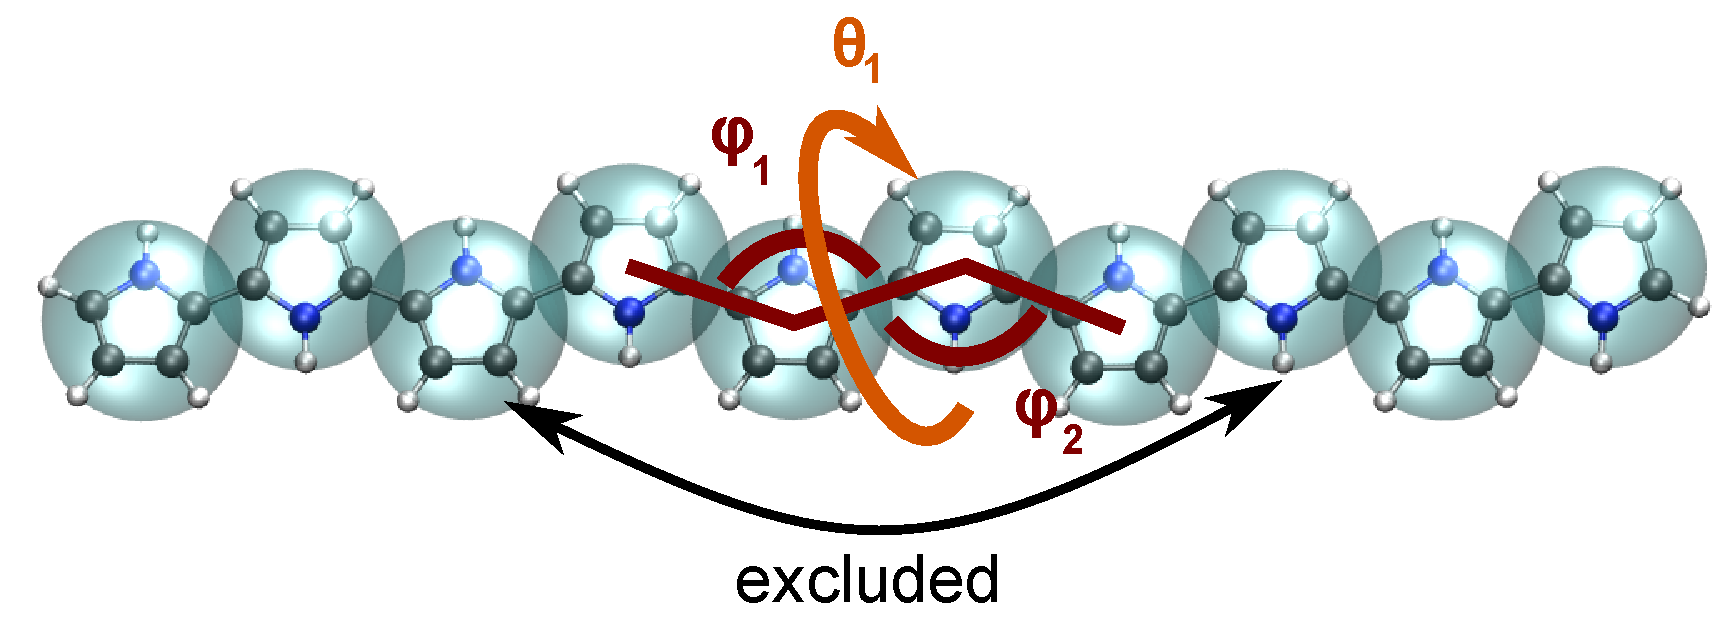
\includegraphics[width=\textwidth]{fig/excl}
  \caption{\label{fig:excl}Example of excluded interactions.}
\end{figure}


%%%%%%%%%%%%%%%%%%%%%%%%%%%%%%%%%%%%%%%%%%%%%%%%%%%%%%%%%%%%%%%%%%%%%%%%%%%%%%%%%%%%%%%%%%%%%%%%
\section{Iterative Boltzmann Inversion}
\label{sec:ibi}

Iterative Boltzmann inversion (\ibi) is a natural extension of the Boltzmann inversion method. Since the goal of the coarse-grained model is to reproduce the distribution functions of the reference system as accurately as possible, one can also iteratively refine the coarse-grained potentials using some numerical scheme.

In \ibi the potential update $\Delta U$ is given by~\cite{Reith:2003}
\begin{eqnarray}
  \label{eq:iter_boltzmann}
  U^{(n+1)} &=& U^{(n)} + \lambda \Delta U^{(n)}~, \\
  \Delta U^{(n)} &=&  k_\text{B} T \ln  \frac{P^{(n)}}{P_{\rm ref}}
  =  U_\text{PMF}^\text{ref} - U_\text{PMF}^{(n)}~.
\end{eqnarray}
Here $\lambda \in (0,1]$ is a numerical factor which helps to stabilize the scheme.

The convergence is reached as soon as the distribution function $P^{(n)}$ matches the reference distribution function $P_{\rm ref}$, or, in other words, the potential of mean force, $U_\text{PMF}^{(n)}$, converges to the reference potential of mean force.

\ibi can be used to refine both bonded and non-bonded potentials. It is primarily used for simple fluids with the aim to reproduce the radial distribution function of the reference system in order to obtain non-bonded interactions. On the implementation side, \ibi has the same issues as the inverse Boltzmann method, i.~e. smoothing and extrapolation of the potential must be used.


\section{Inverse Monte Carlo}
\label{sec:imc}

Inverse Monte Carlo (\imc) is an iterative scheme which additionally includes cross correlations of distributions. A detailed derivation of the \imc method can be found in ref.~\cite{Lyubartsev:1995}.

The potential update $\Delta U$ of the \imc method is calculated by solving a set of linear equations
\begin{align}
    \left<S_{\alpha}\right> - S_{\alpha}^{\text{ref}}= A_{\alpha \gamma} \Delta U_{\gamma}~,
  \label{eq:imc}
\end{align}
%
where
\begin{eqnarray}
  \label{eq:covariance}
  A_{\alpha \gamma} = \frac{\partial \left< S_{\alpha} \right> }{\partial U_{\gamma}}  =
  \beta \left( \left<S_{\alpha} \right>\left<S_{\gamma} \right> - \left<S_{\alpha} S_{\gamma} \right>  \right)~,
  \nonumber
\end{eqnarray}
and $S$ the histogram of a coarse-grained variable of interest. For example, in case of coarse-graining of the non-bonded interactions which depend only on the distance $r_{ij}$ between particles $i$ and $j$ and assuming that the interaction potential is short-ranged, i.e. $U(r_{ij})=0$ if $r_{ij} \ge r_{\text{cut} }$, the average value of $S_{\alpha}$ is related to the radial distribution function $g(r_{\alpha})$ by
%
\begin{equation}
   \left< S_{\alpha} \right> =  \frac{N(N-1)}{2} \frac{4 \pi r_{\alpha}^2 \Delta r} {V}g(r_{\alpha})~,
  \label{eq:s_mean}
\end{equation}
%
where $N$ is the number of atoms in the system ($\frac{1}{2} N(N-1)$ is then the number of all pairs), $\Delta r$ is the grid spacing, $r_{\text{cut}}/M$, $V$ is the total volume of the system. In other words, in this particular case the physical meaning of $S_{\alpha}$ is the number of particle pairs with interparticle distances $r_{ij} = r_{\alpha}$ which correspond to the tabulated value of the potential $U_{\alpha}$.


\section{Force Matching}
\label{sec:fm}

%\sasha

%Brief description with references \\
% Maybe appendix with main equations \\

Force matching (\fm) is another approach to evaluate corse-grained potentials~\cite{Ercolessi:1994,Izvekov:2005,Noid:2007}. In contrast to the structure-based approaches, its aim is not to reproduce various distribution functions, but instead to match the multibody potential of mean force as close as possible with a given set of coarse-grained interactions.

The method works as follows. We first assume that the coarse-grained force-field (and hence the forces) depends on $M$ parameters $g_1,...,g_M $. These parameters can be prefactors of analytical functions, tabulated values of the interaction potentials, or coefficients of splines used to describe these potentials.

In order to determine these parameters, the reference forces on coarse-grained beads are calculated by summing up the forces on the atoms
\begin{equation}
  {\vec F}_I^\text{ref} = \sum_{j \in {\cal S_I}} \frac{d_{Ii}}{c_{Ii}} {\vec f}_j({\vec r^n}),
  \label{eq:force_mapping}
\end{equation}
where the sum is over all atoms of the CG site {\it I} (see. \sect{sec:mapping_operator}).
The $d_{Ij}$ coefficients can, in principle, be chosen arbitrarily, provided that the condition $ \sum_{i=1}^{n}d_{Ii}=1$ is satisfied~\cite{Noid:2008.1}. If mapping coefficients for the forces are not provided, it is assumed that $d_{Ij} = c_{Ij}$ (see also \sect{sec:inputfiles}).

By calculating the reference forces for $L$ snapshots we can write down $N \times L$ equations
%
\begin{equation}
  {\vec F}_{Il}^\text{cg}(g_1, \dots ,g_M)=\vec F_{il}^\text{ref},\;
  I=1,\dots,N,\; l=1,\dots,L~.
  \label{eq:fmatch1}
\end{equation}
%
Here ${\vec F}_{Il}^\text{ref}$ is the force on the bead $I$ and ${\vec F}_{Il}^\text{cg} $ is the coarse-grained representation of this force. The index $l$ enumerates snapshots picked for coarse-graining. By running the simulations long enough one can always ensure that $M < N \times L$. In this case the set of equations~\ref{eq:fmatch1} is overdetermined and can be solved in a least-squares manner.

${\bm F}_{il}^\text{cg}$ is, in principle, a non-linear function of its parameters $\{g_i\}$. Therefore, it is useful to represent the coarse-grained force-field in such a way that equations~(\ref{eq:fmatch1}) become linear functions of $\{g_i\}$. This can be done using splines to describe the functional form of the forces~\cite{Izvekov:2005}. Implementation details are discussed in ref.~\cite{Ruehle:2009.a}.

Note that an adequate sampling of the system requires a large number of snapshots $L$. Hence, the applicability of the method is often constrained by the amount of memory available. To remedy the situation, one can split the trajectory into blocks, find the coarse-grained potential for each block and then perform averaging over all blocks.
